\chapter{Koncepcja systemu Team Challenge}

\begin{comment}
Projekt koncepcyjny? Koncepcja systemu? Systemu NAZWA_WLASNA
\end{comment}

W niniejszym rozdziale zostanie przedstawiony koncept głównych funkcjonalności projektowanego systemu. Podczas pracy koncepcyjnej autor pracy miał na względzie główny cel systemu jakim jest zrzeszanie zawodników. Proponowane funkcjonalności mają umożliwić osiągnięcie tego celu. Tworząc koncept autor kierował się znajomością potrzeb grupy docelowej, której sam jest częścią, a niejednokrotnie swoje pomysły weryfikował z innymi zawodnikami.


System został nazwany Team Challenge. Nazwa ta nawiązuje do głównej funkcjonalności systemu, czyli do wspierania rywalizacji pomiędzy drużynami poprzez rzucanie wyzwań.

  
\section{Baza wiedzy}

W celu umożliwienia zrzeszania zawodników sportów zespołowych konieczne jest przechowywanie w systemie bazy wiedzy na temat zawodników, drużyn oraz obiektów sportowych. W poniższych sekcjach zostaną przybliżone główne założenia dotyczące przechowywania poszczególnych danych.
  
\subsection{Baza zawodników}

Zawodnicy uprawiający amatorsko pewną dyscyplinę sportu są podstawową grupą docelową projektowanego systemu oraz elementem budującym społeczność. Podstawową funkcjonalnością systemu musi być rejestracja zawodników. Podczas procesu rejestracji od użytkownika powinny zostać pobrane dane niezbędne do funkcjonowania systemu, jak również informacje potrzebne do realizacji dalszych założeń, co będzie opisane w kolejnych podpunktach.

\subsection{Baza drużyn}

Zawodnicy po utworzeniu profilu będą mogli założyć drużynę lub dołączyć do już istniejącej drużyny poprzez otrzymanie oraz akceptację zaproszenia. Zawodnik zakładający drużynę otrzymuje specjalną rolę - kapitana. Kapitanem drużyny powinna być osoba reprezentatywna oraz posiadająca dobry kontakt z pozostałymi członkami zespołu, ponieważ to kapitan będzie zajmował się poszukiwaniem przeciwników oraz umawianiem spotkań. Warto zaznaczyć, że kapitan drużyny dalej pozostaje zawodnikiem i może brać czynny udział w rozgrywkach. 

\subsubsection{Punkt macierzysty}

Drużyna powinna wybrać lokalizację, która na potrzeby tej pracy oraz systemu nazwana została "punktem macierzystym". Punkt ten w obrębie systemu będzie służył jako punkt referencyjny dla porównywania odległości pomiędzy drużynami, jak również do oceny odległości od obiektów sportowych. Punktem macierzystym może być na przykład ulubione boisko zawodników lub częste miejsce spotkań pobliskie zawodnikom. W przypadku trudności wyboru domyślną lokalizacją jest centrum regionu, w którym została utworzona drużyna.

\subsubsection{Aktywność drużyny}

Dostęp do kluczowych funkcjonalności takich jak szukanie przeciwników oraz rzucanie wyzwań wymaga posiadania przez drużynę minimalnej liczby zawodników zdefiniowanej dla konkretnej dyscypliny sportu. Drużyna spełniająca powyższy wymóg określana jest mianem drużyny aktywnej.

\subsection{Baza obiektów sportowych}

Mając na uwadze docelową grupę docelową projektowanego systemu jaką są zawodnicy grający amatorsko - system powinien dostarczać bazę obiektów ogólnodostępnych, a przede wszystkim nie wymagających wkładu finansowego. Głównym konceptem w tym zakresie jest umożliwienie zawodnikom zgłaszania oraz weryfikacji obiektów. 

\section{Wspomaganie poszukiwania rywali}

Kluczową funkcjonalnością systemu jest wspomaganie poszukiwania rywali do gry. Projektując tę funkcjonalność autor pracy miał na względzie, że najważniejszym ogniwem w systemie jest korzystający z niego człowiek. Z tego względu system nigdy będzie podejmował decyzji o wyborze przeciwnika samodzielnie. Celem systemu będzie wspieranie tego procesu poprzez dostarczanie kapitanowi propozycji przeciwników na podstawie zdefiniowanych przez niego preferencji.


\subsection{Kryteria dopasowania}

Podstawowym kryterium dopasowywania drużyn będzie maksymalizacja satysfakcji z gry. Poziom satysfakcji stanowi jednak kryterium, które jest wręcz niemożliwe do ustalenia wprost. Z tego powodu zostały zdefiniowane przesłanki, które mogą wpływać na większą satysfakcję drużyn z rozgrywki:

\begin{itemize}
\item{przybliżony wiek zawodników,}
\item{przybliżony poziom umiejętności zawodników,}
\item{przybliżona forma zawodników,}
\item{zachowanie fair-play drużyny przeciwnej,}
\item{dobre wspomnienia po poprzednich rozgrywkach.}
\end{itemize}

Istotne z punktu widzenia kapitana szukającego przeciwników mogą być również czynniki wpływające na możliwość umówienia spotkania. Mogą być to na przykład informacje dotyczące aktywności drużyny przeciwnej, czy na przykład jej preferowane godziny gry.

Przytoczone kryteria powinny zostać uwzględnione w projektowanym mechanizmie wspomaganego wyszukiwania przeciwników. Mechanizm powinien zostać zaimplementowany w sposób rozszerzalny, aby możliwe było definiowanie nowych kryteriów wraz z potrzebami rozwojowymi systemu.

\subsection{Problem optymalizacji wielokryterialnej}

Problem optymalizacji wielokryterialnej jest rozszerzeniem problemu optymalizacji jednokryterialnej, gdzie poszukiwana jest decyzja optymalna, ze zbioru możliwych decyzji na podstawie jednego kryterium. Problem ten sprowadza się do poszukiwania maksimum (bądź minimum) funkcji oceny danego kryterium. Jeżeli kryterium jest ilościowe, np. maksymalna prędkość samochodu, to podejmując decyzje o zakupie jedynie ze względu na to kryterium naturalnie wybierzemy samochód, który osiąga największą prędkość. 

Często jednak podjecie decyzji może być uwarunkowane większą liczbą czynników, na przykład, w przypadku samochodu może to być jego cena, koszt utrzymania, czy czynniki nie ilościowe takie jak jego kolor (w zależności od preferencji kupca). Podejmując decyzje należy rozpatrzyć wiele kryteriów oraz relacje miedzy nimi. Decyzja, która jest optymalna ze względu na jedno z kryteriów, nie musi być optymalna ze względu na pozostałe - z reguły tak nie jest.

\begin{figure}[ht]
\centering
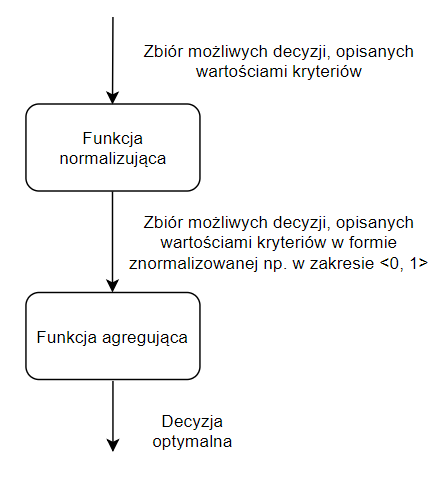
\includegraphics[width=0.5\linewidth]{03-koncept/rys/tradycyjne-algorytmy-opt.PNG}
\caption{Ogólny schemat metody rozwiązywania problemu optymalizacji wielokryterialnej}
\label{fig:diagram-trad-alg-opt}
\end{figure}

Tradycyjnym sposobem rozwiązania problemu jest w pierwszej kolejności znormalizowanie wartości kryteriów do przedziału wartości <0,1>, a następnie dokonanie wyboru korzystając z wybranej funkcji agregującej [?]. Ogólny schemat został przedstawiony na rysunku ~\ref{fig:diagram-trad-alg-opt}

Problem podobnej natury występuje w projektowanym systemie. Poszukiwanie rywali do gry można sprowadzić do poszukiwania najlepszych decyzji wyboru drużyny spośród kwalifikujących się drużyn zdefiniowanych w systemie. Przykładowe kryteria wpływające na wartość funkcji oceny dla poszczególnych decyzji (rywali) zostały zdefiniowane w poprzednim podrozdziale.

\begin{comment}
\subsection{Rozszerzenie tradycyjnego algorytmu}

Proponując algorytm należy mieć na uwadze domenę problemu oraz charakter danych, na jakich będzie on operował. W związku z tym do tradycyjnego schematu oceny rozwiązań zostanie wprowadzona modyfikacja.

 Normalizacja poszczególnych kryteriów będzie przebiegać przy użyciu różnych funkcji, dopasowanych do charakteru danych. Przykładem uzasadniającym konieczność zastosowania takiej modyfikacji może być porównanie dwóch kryteriów: odległości drużyn oraz średniego wieku zawodników. O ile kryterium odległości może być normalizowane w pełni liniowo, o tyle dla różnicy wieku taka metoda normalizacji jest błędna. Różnica wieku między dwoma zawodnikami, którzy mają 15 oraz 20 lat jest znacznie bardziej istotna aniżeli różnica między zawodnikami w wieku 30 oraz 35 lat - nie można tutaj zastosować operatora liniowego. Dodatkowo w domenie problemu można wyróżnić kryteria nieliczbowe - cechy drużyny, które mogą mieć duży wpływ na jakość dopasowania, np. zadeklarowana chęć ponownej gry z daną drużyną.   

\subsection{Metoda ważonych kryteriów}

Metoda ważonych kryteriów polega na opisaniu funkcji oceny decyzji jako sumy ważonej ocen poszczególnych kryteriów [?]. Konieczne jest przyporządkowanie wagi dla każdego z kryteriów. Ocena poszczególnych decyzji obliczana jest według wzoru: 

\begin{equation}\label{eq:mwk}
F(x)=\sum_{i=1}^{k}w_{i}f_{i}(x)
\end{equation}

gdzie k - ilość kryteriów, x - wektor rozwiązań, $w_{i}$ - wagi takie że:

\begin{equation*}
w \in [0, 1] \mbox{ oraz } \sum_{i=1}^{k}w_{i} = 1
\end{equation*}

Metoda ta została wybrana ze względu na możliwość dynamicznego doboru wag poszczególnych kryteriów. Niektóre z tych wag będą dobierane przez kapitana zgodnie z preferencjami jego drużyny. Rysunek~\ref{fig:diagram-alg-ext} przedstawia schemat działania algorytmu przewidzianego w systemie.


\begin{figure}[H]
\centering
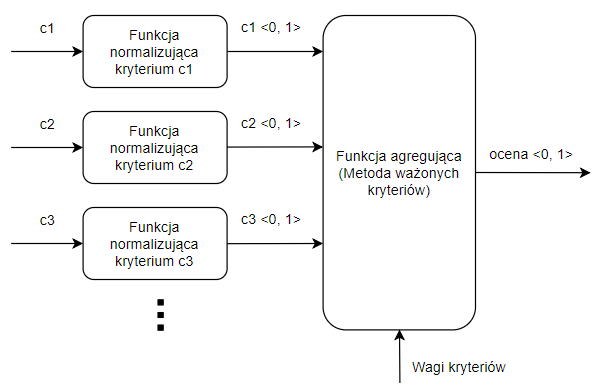
\includegraphics[width=0.8\linewidth]{03-koncept/rys/algorytm.PNG}
\caption{Rozszerzony schemat algorytmu oceny decyzji}
\label{fig:diagram-alg-ext}
\end{figure}
\end{comment}

\section{Wspomaganie umawiania się na rozgrywkę}

Kolejną bazową funkcjonalnością systemu jest wspieranie przebiegu umawiania spotkań. Kapitan aktywnej drużyny może rzucić wyzwanie innej aktywnej drużynie. Kapitan wyzwanej drużyny może podjąć decyzję o odrzuceniu wyzwania. W przeciwnym wypadku rozpoczyna się proces negocjacji terminu oraz miejsca spotkania. 

\subsection{Negocjacja terminu oraz miejsca spotkania}

Kapitanowie drużyn, komunikując się ze swoimi zawodnikami, mogą dodawać do puli ofert swoje propozycje składające się z daty, godziny oraz miejsca spotkania. Miejscem spotkania może być dowolny obiekt sportowy zgłoszony w tym samym regionie co drużyny. System mógłby jednak proponować obiekty położone blisko punktów macierzystych obydwu drużyn. Negocjacje spotkania kończą się w momencie gdy jeden z kapitanów zaakceptuje propozycję drużyny przeciwnej. Termin oraz miejsce zawarte w zaakceptowanej ofercie stają się planowanym terminem oraz miejscem spotkania, a wyzwanie otrzymuje status zaakceptowanego.

\begin{figure}[ht]
\centering
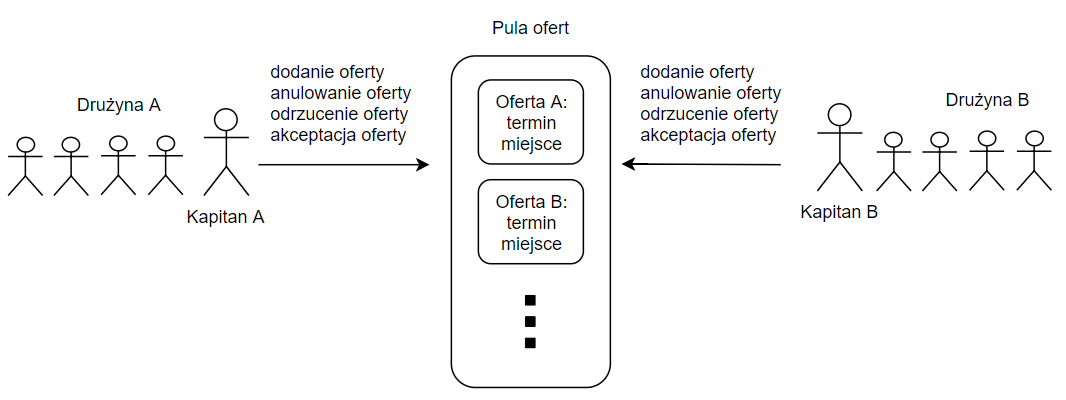
\includegraphics[width=\linewidth]{03-koncept/rys/offer-pool.PNG}
\caption{Konceptualny diagram negocjacji przy użyciu puli ofert}
\label{fig:diagram-alg-ext}
\end{figure}

\subsection{Wyniki spotkań}

Wyzwanie uznaje się za zakończone gdy nastąpi wprowadzenie do systemu jego wyniku. Wynik może zostać wprowadzony przez dowolną z drużyn biorących udział w wyzwaniu. Wprowadzony wynik powinien zostać poddany weryfikacji przez drugiego z kapitanów, który może go potwierdzić, bądź w przypadku niezgodności, odrzucić. Na wynik powinny składać się informacje takie jak: ilość punktów zdobytych przez poszczególne drużyny. W przypadku gdy są to dwie różne liczby wyzwanie kończy się zwycięstwem drużyny, która zdobyła ich więcej. W przeciwnym razie wynikiem wyzwania jest remis.

\subsection{Ocena drużyn}

Kapitanowie drużyn powinni być w stanie dokonać oceny drużyny rywali po zakończonym spotkaniu. Wypełnienie formularza ma na celu dostarczenie do systemu danych, które mogą poprawić jakość wyszukiwania drużyn. Przykładowymi pytaniami mogą być tutaj: ocena poziomu fair-play drużyny oraz deklaracja chęci ponownej rozgrywki w przyszłości. Ze względu na umożliwienie swobodnej oraz szczerej odpowiedzi oceny nie mogą być widoczne dla ocenianych drużyn.
